\begin{figure}[htbp]
\centering
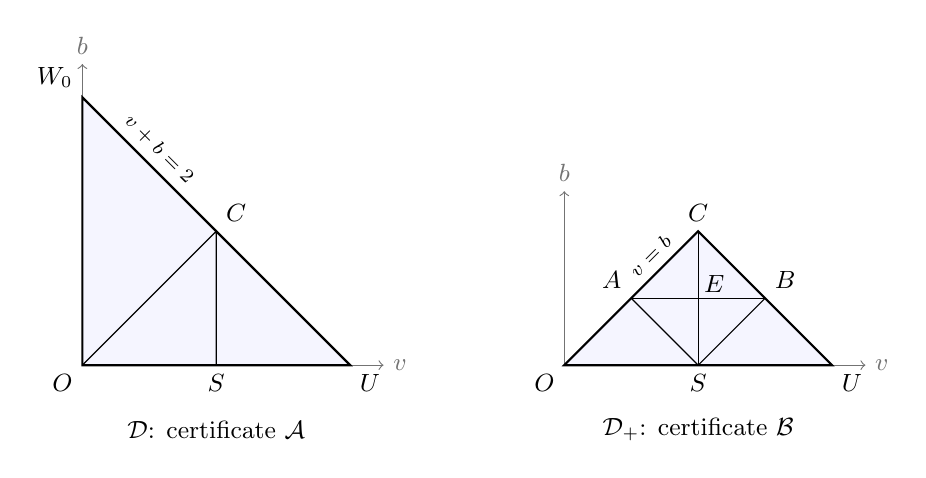
\begin{tikzpicture}[scale=1.7, every node/.style={font=\small}]
 \begin{scope}
  \fill[blue!4] (0,0)--(2,0)--(0,2)--cycle;
  \draw[->,black!55] (0,0)--(2.25,0) node[right] {$v$};
  \draw[->,black!55] (0,0)--(0,2.25) node[above] {$b$};
  \draw[thick] (0,0)--(2,0)--(0,2)--cycle;
  \path (2,0)--(0,2) node[pos=.76,above,sloped,font=\scriptsize]
    {$v+b=2$};
  \draw (0,0)--(1,1)--(1,0);
  \node[below left] at (0,0) {$O$};
  \node[below] at (1,0) {$S$};
  \node[below right] at (2,0) {$U$};
  \node[above right] at (1,1) {$C$};
  \node[above left] at (0,2) {$W_0$};
  \node at (1,-0.48) {$\mathcal D$: certificate $\mathcal A$};
 \end{scope}
 \begin{scope}[xshift=3.6cm]
  \fill[blue!4] (0,0)--(2,0)--(1,1)--cycle;
  \draw[->,black!55] (0,0)--(2.25,0) node[right] {$v$};
  \draw[->,black!55] (0,0)--(0,1.3) node[above] {$b$};
  \draw[thick] (0,0)--(2,0)--(1,1)--cycle;
  \path (0,0)--(1,1) node[pos=.73,above,sloped,font=\scriptsize]
    {$v=b$};
  \draw (0.5,0.5)--(1,0)--(1.5,0.5);
  \draw (1,0)--(1,1);
  \draw (0.5,0.5)--(1.5,0.5);
  \node[below left] at (0,0) {$O$};
  \node[below] at (1,0) {$S$};
  \node[below right] at (2,0) {$U$};
  \node[above] at (1,1) {$C$};
  \node[above left] at (0.5,0.5) {$A$};
  \node[above right] at (1.5,0.5) {$B$};
  \node[above right,inner sep=2pt] at (1,0.5) {$E$};
  \node at (1,-0.48) {$\mathcal D_+$: certificate $\mathcal B$};
 \end{scope}
\end{tikzpicture}
\caption{Subdivisions of the Weyl-norm domains
$\mathcal D=\{(v,b):v,b\ge0,\ v+b\le2\}$ and
$\mathcal D_+=\mathcal D\cap\{v\ge b\}$ used in the triangular
coefficient table. Every edge is included. The norm condition
$v+b\le2$ is a necessary relaxation of the sectional-curvature condition;
the tensor estimates retain the stronger constraint $x+y\le2$.}
\label{fig:certificate-domains}
\end{figure}
